%-*-latex-*-
\tinysidebar{\debug{exercises/3n3-5-42-n5-n2-1/main.tex}}
The following are plots of $|f(n)|$ and $g(n) = n^4$:
%-*-latex-*-

\begin{center}
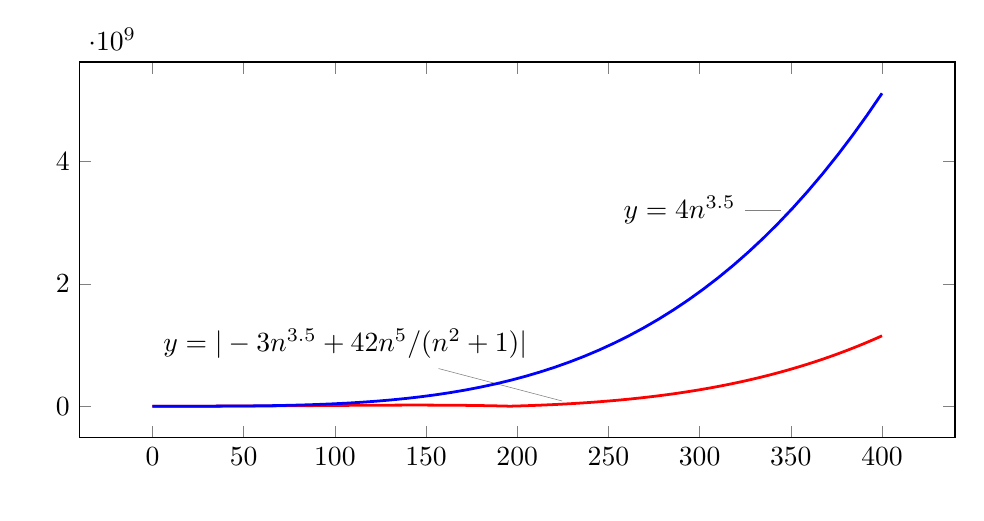
\begin{tikzpicture}[line width=1]
\begin{axis}[width=5in, height=2.5in,
             scatter/classes={a={mark=*,draw=black}},
             xlabel={\mbox{}},
             xlabel style={name=xlabel}, 
             ylabel={\mbox{}}, 
             legend style={
                at={(xlabel.south)},
                yshift=-1ex,
                anchor=north,
                legend cell align=left,
                },
        ]
]
\addplot[draw=red, line width=1] coordinates {(0.0,0.0)
(0.4004,0.2507)
(0.8008,7.0486)
(1.2012,37.297)
(1.6016,108.5522)
(2.002,235.6557)
(2.4024,431.8796)
(2.8028,709.7459)
(3.2032,1081.3376)
(3.6036,1558.4105)
(4.004,2152.4386)
(4.4044,2874.6353)
(4.8048,3735.9684)
(5.2052,4747.1701)
(5.6056,5918.7465)
(6.006,7260.9853)
(6.4064,8783.9631)
(6.8068,10497.5521)
(7.2072,12411.426)
(7.6076,14535.0659)
(8.008,16877.7652)
(8.4084,19448.6346)
(8.8088,22256.6065)
(9.2092,25310.4394)
(9.6096,28618.7215)
(10.01,32189.8746)
(10.4104,36032.1575)
(10.8108,40153.6692)
(11.2112,44562.3521)
(11.6116,49265.9949)
(12.012,54272.235)
(12.4124,59588.5617)
(12.8128,65222.3182)
(13.2132,71180.7041)
(13.6136,77470.7779)
(14.014,84099.4586)
(14.4144,91073.5285)
(14.8148,98399.6344)
(15.2152,106084.29)
(15.6156,114133.8776)
(16.016,122554.6497)
(16.4164,131352.7307)
(16.8168,140534.1188)
(17.2172,150104.6871)
(17.6176,160070.1855)
(18.018,170436.2418)
(18.4184,181208.3632)
(18.8188,192391.938)
(19.2192,203992.2363)
(19.6196,216014.4116)
(20.02,228463.5021)
(20.4204,241344.4317)
(20.8208,254662.0111)
(21.2212,268420.9393)
(21.6216,282625.8042)
(22.022,297281.0837)
(22.4224,312391.1473)
(22.8228,327960.2563)
(23.2232,343992.5653)
(23.6236,360492.1229)
(24.024,377462.8729)
(24.4244,394908.6546)
(24.8248,412833.2045)
(25.2252,431240.1564)
(25.6256,450133.0427)
(26.026,469515.2949)
(26.4264,489390.2447)
(26.8268,509761.1245)
(27.2272,530631.0684)
(27.6276,552003.1126)
(28.028,573880.1964)
(28.4284,596265.1629)
(28.8288,619160.7596)
(29.2292,642569.6391)
(29.6296,666494.3596)
(30.03,690937.3859)
(30.4304,715901.0898)
(30.8308,741387.7506)
(31.2312,767399.556)
(31.6316,793938.6027)
(32.032,821006.8966)
(32.4324,848606.3537)
(32.8328,876738.8007)
(33.2332,905405.9753)
(33.6336,934609.5269)
(34.034,964351.0174)
(34.4344,994631.921)
(34.8348,1025453.6255)
(35.2352,1056817.4323)
(35.6356,1088724.5571)
(36.036,1121176.1304)
(36.4364,1154173.1979)
(36.8368,1187716.721)
(37.2372,1221807.5772)
(37.6376,1256446.5608)
(38.038,1291634.3831)
(38.4384,1327371.6727)
(38.8388,1363658.9765)
(39.2392,1400496.7596)
(39.6396,1437885.4059)
(40.04,1475825.2186)
(40.4404,1514316.4203)
(40.8408,1553359.154)
(41.2412,1592953.4829)
(41.6416,1633099.3909)
(42.042,1673796.7834)
(42.4424,1715045.4872)
(42.8428,1756845.2511)
(43.2432,1799195.7462)
(43.6436,1842096.5662)
(44.044,1885547.2282)
(44.4444,1929547.1722)
(44.8448,1974095.7624)
(45.2452,2019192.2869)
(45.6456,2064835.9581)
(46.046,2111025.9135)
(46.4464,2157761.2154)
(46.8468,2205040.8516)
(47.2472,2252863.7359)
(47.6476,2301228.7077)
(48.048,2350134.5333)
(48.4484,2399579.9052)
(48.8488,2449563.4433)
(49.2492,2500083.6946)
(49.6496,2551139.1338)
(50.0501,2602728.1633)
(50.4505,2654849.1138)
(50.8509,2707500.2446)
(51.2513,2760679.7437)
(51.6517,2814385.7279)
(52.0521,2868616.2436)
(52.4525,2923369.2667)
(52.8529,2978642.7029)
(53.2533,3034434.3882)
(53.6537,3090742.0887)
(54.0541,3147563.5015)
(54.4545,3204896.2544)
(54.8549,3262737.9064)
(55.2553,3321085.9479)
(55.6557,3379937.8012)
(56.0561,3439290.8202)
(56.4565,3499142.2912)
(56.8569,3559489.4329)
(57.2573,3620329.3965)
(57.6577,3681659.2661)
(58.0581,3743476.0592)
(58.4585,3805776.7265)
(58.8589,3868558.152)
(59.2593,3931817.154)
(59.6597,3995550.4846)
(60.0601,4059754.83)
(60.4605,4124426.8113)
(60.8609,4189562.984)
(61.2613,4255159.8386)
(61.6617,4321213.8007)
(62.0621,4387721.2313)
(62.4625,4454678.427)
(62.8629,4522081.62)
(63.2633,4589926.9786)
(63.6637,4658210.6074)
(64.0641,4726928.5471)
(64.4645,4796076.7752)
(64.8649,4865651.2058)
(65.2653,4935647.6902)
(65.6657,5006062.0167)
(66.0661,5076889.9109)
(66.4665,5148127.0362)
(66.8669,5219768.9936)
(67.2673,5291811.322)
(67.6677,5364249.4984)
(68.0681,5437078.9383)
(68.4685,5510294.9954)
(68.8689,5583892.9623)
(69.2693,5657868.0704)
(69.6697,5732215.4899)
(70.0701,5806930.3305)
(70.4705,5882007.6412)
(70.8709,5957442.4104)
(71.2713,6033229.5664)
(71.6717,6109363.9774)
(72.0721,6185840.4513)
(72.4725,6262653.7368)
(72.8729,6339798.5226)
(73.2733,6417269.438)
(73.6737,6495061.0531)
(74.0741,6573167.8789)
(74.4745,6651584.3674)
(74.8749,6730304.9119)
(75.2753,6809323.8469)
(75.6757,6888635.4485)
(76.0761,6968233.9344)
(76.4765,7048113.4644)
(76.8769,7128268.14)
(77.2773,7208692.005)
(77.6777,7289379.0453)
(78.0781,7370323.1894)
(78.4785,7451518.3083)
(78.8789,7532958.2159)
(79.2793,7614636.6688)
(79.6797,7696547.3666)
(80.0801,7778683.9523)
(80.4805,7861040.0119)
(80.8809,7943609.075)
(81.2813,8026384.615)
(81.6817,8109360.0487)
(82.0821,8192528.7369)
(82.4825,8275883.9844)
(82.8829,8359419.0403)
(83.2833,8443127.0978)
(83.6837,8527001.2945)
(84.0841,8611034.7126)
(84.4845,8695220.3792)
(84.8849,8779551.2658)
(85.2853,8864020.2892)
(85.6857,8948620.3111)
(86.0861,9033344.1384)
(86.4865,9118184.5235)
(86.8869,9203134.1641)
(87.2873,9288185.7035)
(87.6877,9373331.7307)
(88.0881,9458564.7808)
(88.4885,9543877.3344)
(88.8889,9629261.8185)
(89.2893,9714710.6064)
(89.6897,9800216.0173)
(90.0901,9885770.3174)
(90.4905,9971365.719)
(90.8909,10056994.3813)
(91.2913,10142648.4103)
(91.6917,10228319.8589)
(92.0921,10314000.727)
(92.4925,10399682.9618)
(92.8929,10485358.4575)
(93.2933,10571019.056)
(93.6937,10656656.5465)
(94.0941,10742262.6659)
(94.4945,10827829.0986)
(94.8949,10913347.4772)
(95.2953,10998809.382)
(95.6957,11084206.3414)
(96.0961,11169529.832)
(96.4965,11254771.2787)
(96.8969,11339922.0545)
(97.2973,11424973.4814)
(97.6977,11509916.8295)
(98.0981,11594743.318)
(98.4985,11679444.1145)
(98.8989,11764010.3359)
(99.2993,11848433.0479)
(99.6997,11932703.2653)
(100.1001,12016811.9521)
(100.5005,12100750.0219)
(100.9009,12184508.3374)
(101.3013,12268077.7109)
(101.7017,12351448.9045)
(102.1021,12434612.6298)
(102.5025,12517559.5483)
(102.9029,12600280.2715)
(103.3033,12682765.3608)
(103.7037,12765005.3278)
(104.1041,12846990.6342)
(104.5045,12928711.6922)
(104.9049,13010158.8643)
(105.3053,13091322.4635)
(105.7057,13172192.7533)
(106.1061,13252759.9481)
(106.5065,13333014.2129)
(106.9069,13412945.6636)
(107.3073,13492544.3672)
(107.7077,13571800.3416)
(108.1081,13650703.556)
(108.5085,13729243.9307)
(108.9089,13807411.3374)
(109.3093,13885195.5992)
(109.7097,13962586.4908)
(110.1101,14039573.7384)
(110.5105,14116147.0199)
(110.9109,14192295.9649)
(111.3113,14268010.1551)
(111.7117,14343279.124)
(112.1121,14418092.3571)
(112.5125,14492439.2921)
(112.9129,14566309.3189)
(113.3133,14639691.7795)
(113.7137,14712575.9687)
(114.1141,14784951.1334)
(114.5145,14856806.4732)
(114.9149,14928131.1403)
(115.3153,14998914.2395)
(115.7157,15069144.8286)
(116.1161,15138811.9182)
(116.5165,15207904.4718)
(116.9169,15276411.406)
(117.3173,15344321.5905)
(117.7177,15411623.8482)
(118.1181,15478306.9553)
(118.5185,15544359.6414)
(118.9189,15609770.5893)
(119.3193,15674528.4357)
(119.7197,15738621.7707)
(120.1201,15802039.1379)
(120.5205,15864769.035)
(120.9209,15926799.9133)
(121.3213,15988120.1781)
(121.7217,16048718.1886)
(122.1221,16108582.2582)
(122.5225,16167700.6542)
(122.9229,16226061.5984)
(123.3233,16283653.2667)
(123.7237,16340463.7894)
(124.1241,16396481.2512)
(124.5245,16451693.6913)
(124.9249,16506089.1036)
(125.3253,16559655.4365)
(125.7257,16612380.5933)
(126.1261,16664252.432)
(126.5265,16715258.7654)
(126.9269,16765387.3613)
(127.3273,16814625.9425)
(127.7277,16862962.187)
(128.1281,16910383.7279)
(128.5285,16956878.1534)
(128.9289,17002433.0071)
(129.3293,17047035.788)
(129.7297,17090673.9505)
(130.1301,17133334.9044)
(130.5305,17175006.0152)
(130.9309,17215674.6041)
(131.3313,17255327.9478)
(131.7317,17293953.2789)
(132.1321,17331537.786)
(132.5325,17368068.6132)
(132.9329,17403532.861)
(133.3333,17437917.5858)
(133.7337,17471209.8)
(134.1341,17503396.4722)
(134.5345,17534464.5275)
(134.9349,17564400.8469)
(135.3353,17593192.2681)
(135.7357,17620825.5851)
(136.1361,17647287.5485)
(136.5365,17672564.8653)
(136.9369,17696644.1992)
(137.3373,17719512.1708)
(137.7377,17741155.357)
(138.1381,17761560.2921)
(138.5385,17780713.4667)
(138.9389,17798601.3288)
(139.3393,17815210.2832)
(139.7397,17830526.6918)
(140.1401,17844536.8737)
(140.5405,17857227.105)
(140.9409,17868583.6193)
(141.3413,17878592.6073)
(141.7417,17887240.2173)
(142.1421,17894512.5548)
(142.5425,17900395.683)
(142.9429,17904875.6225)
(143.3433,17907938.3516)
(143.7437,17909569.8063)
(144.1441,17909755.8803)
(144.5445,17908482.4251)
(144.9449,17905735.2499)
(145.3453,17901500.1222)
(145.7457,17895762.767)
(146.1461,17888508.8677)
(146.5465,17879724.0655)
(146.9469,17869393.96)
(147.3473,17857504.1088)
(147.7477,17844040.0279)
(148.1481,17828987.1915)
(148.5485,17812331.0323)
(148.9489,17794056.9412)
(149.3493,17774150.2678)
(149.7497,17752596.3201)
(150.1502,17729380.3649)
(150.5506,17704487.6274)
(150.951,17677903.2917)
(151.3514,17649612.5004)
(151.7518,17619600.3552)
(152.1522,17587851.9166)
(152.5526,17554352.2038)
(152.953,17519086.1954)
(153.3534,17482038.8285)
(153.7538,17443194.9998)
(154.1542,17402539.5648)
(154.5546,17360057.3383)
(154.955,17315733.0944)
(155.3554,17269551.5663)
(155.7558,17221497.4468)
(156.1562,17171555.3879)
(156.5566,17119710.0012)
(156.957,17065945.8578)
(157.3574,17010247.4882)
(157.7578,16952599.3827)
(158.1582,16892985.9911)
(158.5586,16831391.723)
(158.959,16767800.9479)
(159.3594,16702197.9947)
(159.7598,16634567.1526)
(160.1602,16564892.6705)
(160.5606,16493158.7574)
(160.961,16419349.5821)
(161.3614,16343449.2736)
(161.7618,16265441.9211)
(162.1622,16185311.5738)
(162.5626,16103042.2412)
(162.963,16018617.893)
(163.3634,15932022.4594)
(163.7638,15843239.8306)
(164.1642,15752253.8577)
(164.5646,15659048.3518)
(164.965,15563607.0847)
(165.3654,15465913.7888)
(165.7658,15365952.1571)
(166.1662,15263705.8431)
(166.5666,15159158.4611)
(166.967,15052293.5862)
(167.3674,14943094.7542)
(167.7678,14831545.4619)
(168.1682,14717629.1666)
(168.5686,14601329.287)
(168.969,14482629.2025)
(169.3694,14361512.2537)
(169.7698,14237961.742)
(170.1702,14111960.9301)
(170.5706,13983493.042)
(170.971,13852541.2626)
(171.3714,13719088.7384)
(171.7718,13583118.5768)
(172.1722,13444613.8469)
(172.5726,13303557.5789)
(172.973,13159932.7648)
(173.3734,13013722.3578)
(173.7738,12864909.2725)
(174.1742,12713476.3855)
(174.5746,12559406.5347)
(174.975,12402682.5197)
(175.3754,12243287.1019)
(175.7758,12081203.0043)
(176.1762,11916412.9117)
(176.5766,11748899.471)
(176.977,11578645.2907)
(177.3774,11405632.9412)
(177.7778,11229844.955)
(178.1782,11051263.8267)
(178.5786,10869872.0127)
(178.979,10685651.9316)
(179.3794,10498585.9641)
(179.7798,10308656.4532)
(180.1802,10115845.704)
(180.5806,9920135.984)
(180.981,9721509.5227)
(181.3814,9519948.5122)
(181.7818,9315435.107)
(182.1822,9107951.4239)
(182.5826,8897479.5422)
(182.983,8684001.5038)
(183.3834,8467499.3131)
(183.7838,8247954.9369)
(184.1842,8025350.305)
(184.5846,7799667.3096)
(184.985,7570887.8057)
(185.3854,7338993.611)
(185.7858,7103966.5061)
(186.1862,6865788.2344)
(186.5866,6624440.5022)
(186.987,6379904.9785)
(187.3874,6132163.2956)
(187.7878,5881197.0485)
(188.1882,5626987.7954)
(188.5886,5369517.0575)
(188.989,5108766.3193)
(189.3894,4844717.028)
(189.7898,4577350.5946)
(190.1902,4306648.3928)
(190.5906,4032591.7598)
(190.991,3755161.9962)
(191.3914,3474340.3658)
(191.7918,3190108.0958)
(192.1922,2902446.3768)
(192.5926,2611336.363)
(192.993,2316759.172)
(193.3934,2018695.8849)
(193.7938,1717127.5464)
(194.1942,1412035.1649)
(194.5946,1103399.7123)
(194.995,791202.1243)
(195.3954,475423.3003)
(195.7958,156044.1035)
(196.1962,166954.6391)
(196.5966,493592.1369)
(196.997,823887.635)
(197.3974,1157860.415)
(197.7978,1495529.7943)
(198.1982,1836915.1264)
(198.5986,2182035.8007)
(198.999,2530911.2427)
(199.3994,2883560.9138)
(199.7998,3240004.311)
(200.2002,3600260.9674)
(200.6006,3964350.4518)
(201.001,4332292.3689)
(201.4014,4704106.3589)
(201.8018,5079812.0979)
(202.2022,5459429.2975)
(202.6026,5842977.705)
(203.003,6230477.1032)
(203.4034,6621947.3107)
(203.8038,7017408.1813)
(204.2042,7416879.6044)
(204.6046,7820381.5049)
(205.005,8227933.8431)
(205.4054,8639556.6147)
(205.8058,9055269.8506)
(206.2062,9475093.6171)
(206.6066,9899048.0158)
(207.007,10327153.1835)
(207.4074,10759429.2922)
(207.8078,11195896.5491)
(208.2082,11636575.1966)
(208.6086,12081485.512)
(209.009,12530647.8078)
(209.4094,12984082.4316)
(209.8098,13441809.7659)
(210.2102,13903850.2283)
(210.6106,14370224.271)
(211.011,14840952.3815)
(211.4114,15316055.082)
(211.8118,15795552.9294)
(212.2122,16279466.5157)
(212.6126,16767816.4674)
(213.013,17260623.446)
(213.4134,17757908.1473)
(213.8138,18259691.3022)
(214.2142,18765993.676)
(214.6146,19276836.0687)
(215.015,19792239.3148)
(215.4154,20312224.2834)
(215.8158,20836811.878)
(216.2162,21366023.0368)
(216.6166,21899878.7322)
(217.017,22438399.9712)
(217.4174,22981607.795)
(217.8178,23529523.2794)
(218.2182,24082167.5343)
(218.6186,24639561.7039)
(219.019,25201726.9667)
(219.4194,25768684.5356)
(219.8198,26340455.6574)
(220.2202,26917061.6132)
(220.6206,27498523.7182)
(221.021,28084863.3218)
(221.4214,28676101.8073)
(221.8218,29272260.5922)
(222.2222,29873361.1278)
(222.6226,30479424.8997)
(223.023,31090473.4271)
(223.4234,31706528.2633)
(223.8238,32327610.9954)
(224.2242,32953743.2445)
(224.6246,33584946.6654)
(225.025,34221242.9466)
(225.4254,34862653.8107)
(225.8258,35509201.0136)
(226.2262,36160906.3453)
(226.6266,36817791.6291)
(227.027,37479878.7223)
(227.4274,38147189.5155)
(227.8278,38819745.9332)
(228.2282,39497569.9331)
(228.6286,40180683.5068)
(229.029,40869108.679)
(229.4294,41562867.5082)
(229.8298,42261982.0862)
(230.2302,42966474.5382)
(230.6306,43676367.0228)
(231.031,44391681.7319)
(231.4314,45112440.8908)
(231.8318,45838666.758)
(232.2322,46570381.6254)
(232.6326,47307607.8181)
(233.033,48050367.6941)
(233.4334,48798683.6451)
(233.8338,49552578.0956)
(234.2342,50312073.5033)
(234.6346,51077192.3589)
(235.035,51847957.1863)
(235.4354,52624390.5425)
(235.8358,53406515.0173)
(236.2362,54194353.2336)
(236.6366,54987927.8472)
(237.037,55787261.5469)
(237.4374,56592377.0543)
(237.8378,57403297.1239)
(238.2382,58220044.5431)
(238.6386,59042642.1321)
(239.039,59871112.7437)
(239.4394,60705479.2637)
(239.8398,61545764.6105)
(240.2402,62391991.7352)
(240.6406,63244183.6217)
(241.041,64102363.2865)
(241.4414,64966553.7785)
(241.8418,65836778.1794)
(242.2422,66713059.6036)
(242.6426,67595421.1977)
(243.043,68483886.141)
(243.4434,69378477.6454)
(243.8438,70279218.955)
(244.2442,71186133.3465)
(244.6446,72099244.129)
(245.045,73018574.6439)
(245.4454,73944148.265)
(245.8458,74875988.3984)
(246.2462,75814118.4825)
(246.6466,76758561.9881)
(247.047,77709342.4181)
(247.4474,78666483.3076)
(247.8478,79630008.224)
(248.2482,80599940.7669)
(248.6486,81576304.5678)
(249.049,82559123.2906)
(249.4494,83548420.6311)
(249.8498,84544220.3172)
(250.2503,85546546.109)
(250.6507,86555421.7985)
(251.0511,87570871.2096)
(251.4515,88592918.1982)
(251.8519,89621586.6522)
(252.2523,90656900.4914)
(252.6527,91698883.6675)
(253.0531,92747560.164)
(253.4535,93802953.9963)
(253.8539,94865089.2116)
(254.2543,95933989.8887)
(254.6547,97009680.1385)
(255.0551,98092184.1034)
(255.4555,99181525.9575)
(255.8559,100277729.9067)
(256.2563,101380820.1886)
(256.6567,102490821.0722)
(257.0571,103607756.8584)
(257.4575,104731651.8794)
(257.8579,105862530.4991)
(258.2583,107000417.1131)
(258.6587,108145336.1482)
(259.0591,109297312.0629)
(259.4595,110456369.3471)
(259.8599,111622532.5222)
(260.2603,112795826.1409)
(260.6607,113976274.7873)
(261.0611,115163903.0769)
(261.4615,116358735.6567)
(261.8619,117560797.2048)
(262.2623,118770112.4306)
(262.6627,119986706.075)
(263.0631,121210602.9098)
(263.4635,122441827.7383)
(263.8639,123680405.3949)
(264.2643,124926360.7452)
(264.6647,126179718.686)
(265.0651,127440504.145)
(265.4655,128708742.0812)
(265.8659,129984457.4848)
(266.2663,131267675.3767)
(266.6667,132558420.8092)
(267.0671,133856718.8653)
(267.4675,135162594.6593)
(267.8679,136476073.3362)
(268.2683,137797180.072)
(268.6687,139125940.0738)
(269.0691,140462378.5794)
(269.4695,141806520.8574)
(269.8699,143158392.2076)
(270.2703,144518017.9602)
(270.6707,145885423.4764)
(271.0711,147260634.1484)
(271.4715,148643675.3987)
(271.8719,150034572.6809)
(272.2723,151433351.4792)
(272.6727,152840037.3084)
(273.0731,154254655.7141)
(273.4735,155677232.2724)
(273.8739,157107792.5903)
(274.2743,158546362.305)
(274.6747,159992967.0846)
(275.0751,161447632.6275)
(275.4755,162910384.663)
(275.8759,164381248.9505)
(276.2763,165860251.2802)
(276.6767,167347417.4725)
(277.0771,168842773.3784)
(277.4775,170346344.8794)
(277.8779,171858157.8873)
(278.2783,173378238.3441)
(278.6787,174906612.2225)
(279.0791,176443305.5253)
(279.4795,177988344.2858)
(279.8799,179541754.5673)
(280.2803,181103562.4636)
(280.6807,182673794.0987)
(281.0811,184252475.6268)
(281.4815,185839633.2324)
(281.8819,187435293.1299)
(282.2823,189039481.5643)
(282.6827,190652224.8103)
(283.0831,192273549.173)
(283.4835,193903480.9875)
(283.8839,195542046.619)
(284.2843,197189272.4627)
(284.6847,198845184.944)
(285.0851,200509810.518)
(285.4855,202183175.6701)
(285.8859,203865306.9155)
(286.2863,205556230.7995)
(286.6867,207255973.8971)
(287.0871,208964562.8133)
(287.4875,210682024.1832)
(287.8879,212408384.6714)
(288.2883,214143670.9726)
(288.6887,215887909.8112)
(289.0891,217641127.9416)
(289.4895,219403352.1476)
(289.8899,221174609.2432)
(290.2903,222954926.0718)
(290.6907,224744329.5068)
(291.0911,226542846.451)
(291.4915,228350503.8371)
(291.8919,230167328.6274)
(292.2923,231993347.8138)
(292.6927,233828588.4179)
(293.0931,235673077.4908)
(293.4935,237526842.1133)
(293.8939,239389909.3956)
(294.2943,241262306.4775)
(294.6947,243144060.5285)
(295.0951,245035198.7472)
(295.4955,246935748.3621)
(295.8959,248845736.6309)
(296.2963,250765190.8408)
(296.6967,252694138.3084)
(297.0971,254632606.3798)
(297.4975,256580622.4303)
(297.8979,258538213.8647)
(298.2983,260505408.1171)
(298.6987,262482232.6509)
(299.0991,264468714.9588)
(299.4995,266464882.5628)
(299.8999,268470763.0141)
(300.3003,270486383.8933)
(300.7007,272511772.81)
(301.1011,274546957.4031)
(301.5015,276591965.3407)
(301.9019,278646824.3202)
(302.3023,280711562.0677)
(302.7027,282786206.339)
(303.1031,284870784.9186)
(303.5035,286965325.6201)
(303.9039,289069856.2864)
(304.3043,291184404.7893)
(304.7047,293308999.0296)
(305.1051,295443666.9372)
(305.5055,297588436.4709)
(305.9059,299743335.6185)
(306.3063,301908392.3968)
(306.7067,304083634.8514)
(307.1071,306269091.057)
(307.5075,308464789.117)
(307.9079,310670757.1638)
(308.3083,312887023.3587)
(308.7087,315113615.8918)
(309.1091,317350562.9818)
(309.5095,319597892.8765)
(309.9099,321855633.8524)
(310.3103,324123814.2146)
(310.7107,326402462.2972)
(311.1111,328691606.4628)
(311.5115,330991275.1029)
(311.9119,333301496.6375)
(312.3123,335622299.5155)
(312.7127,337953712.2142)
(313.1131,340295763.2396)
(313.5135,342648481.1265)
(313.9139,345011894.4381)
(314.3143,347386031.7662)
(314.7147,349770921.7313)
(315.1151,352166592.9823)
(315.5155,354573074.1966)
(315.9159,356990394.0802)
(316.3163,359418581.3676)
(316.7167,361857664.8218)
(317.1171,364307673.234)
(317.5175,366768635.4242)
(317.9179,369240580.2404)
(318.3183,371723536.5595)
(318.7187,374217533.2863)
(319.1191,376722599.3543)
(319.5195,379238763.7251)
(319.9199,381766055.3889)
(320.3203,384304503.3639)
(320.7207,386854136.6968)
(321.1211,389414984.4625)
(321.5215,391987075.7642)
(321.9219,394570439.7333)
(322.3223,397165105.5294)
(322.7227,399771102.3403)
(323.1231,402388459.3821)
(323.5235,405017205.899)
(323.9239,407657371.1632)
(324.3243,410308984.4753)
(324.7247,412972075.1638)
(325.1251,415646672.5855)
(325.5255,418332806.125)
(325.9259,421030505.1952)
(326.3263,423739799.2371)
(326.7267,426460717.7194)
(327.1271,429193290.139)
(327.5275,431937546.021)
(327.9279,434693514.9182)
(328.3283,437461226.4114)
(328.7287,440240710.1095)
(329.1291,443031995.6491)
(329.5295,445835112.6948)
(329.9299,448650090.9392)
(330.3303,451476960.1027)
(330.7307,454315749.9336)
(331.1311,457166490.2078)
(331.5315,460029210.7294)
(331.9319,462903941.3301)
(332.3323,465790711.8693)
(332.7327,468689552.2345)
(333.1331,471600492.3405)
(333.5335,474523562.1303)
(333.9339,477458791.5743)
(334.3343,480406210.6707)
(334.7347,483365849.4455)
(335.1351,486337737.9523)
(335.5355,489321906.2723)
(335.9359,492318384.5143)
(336.3363,495327202.815)
(336.7367,498348391.3383)
(337.1371,501381980.2761)
(337.5375,504427999.8476)
(337.9379,507486480.2997)
(338.3383,510557451.9067)
(338.7387,513640944.9705)
(339.1391,516736989.8207)
(339.5395,519845616.8141)
(339.9399,522966856.335)
(340.3403,526100738.7955)
(340.7407,529247294.6347)
(341.1411,532406554.3194)
(341.5415,535578548.3438)
(341.9419,538763307.2293)
(342.3423,541960861.525)
(342.7427,545171241.807)
(343.1431,548394478.6792)
(343.5435,551630602.7723)
(343.9439,554879644.7447)
(344.3443,558141635.282)
(344.7447,561416605.0971)
(345.1451,564704584.9301)
(345.5455,568005605.5483)
(345.9459,571319697.7465)
(346.3463,574646892.3465)
(346.7467,577987220.1973)
(347.1471,581340712.1753)
(347.5475,584707399.1837)
(347.9479,588087312.1533)
(348.3483,591480482.0417)
(348.7487,594886939.8338)
(349.1491,598306716.5415)
(349.5495,601739843.204)
(349.9499,605186350.8873)
(350.3504,608646270.6847)
(350.7508,612119633.7165)
(351.1512,615606471.1299)
(351.5516,619106814.0992)
(351.952,622620693.8258)
(352.3524,626148141.5379)
(352.7528,629689188.4909)
(353.1532,633243865.967)
(353.5536,636812205.2754)
(353.954,640394237.7521)
(354.3544,643989994.7602)
(354.7548,647599507.6896)
(355.1552,651222807.9571)
(355.5556,654859927.0063)
(355.956,658510896.3078)
(356.3564,662175747.3589)
(356.7568,665854511.6838)
(357.1572,669547220.8334)
(357.5576,673253906.3855)
(357.958,676974599.9447)
(358.3584,680709333.1423)
(358.7588,684458137.6362)
(359.1592,688221045.1114)
(359.5596,691998087.2792)
(359.96,695789295.8778)
(360.3604,699594702.6722)
(360.7608,703414339.4539)
(361.1612,707248238.0411)
(361.5616,711096430.2786)
(361.962,714958948.038)
(362.3624,718835823.2173)
(362.7628,722727087.7411)
(363.1632,726632773.5608)
(363.5636,730552912.6543)
(363.964,734487537.0257)
(364.3644,738436678.7063)
(364.7648,742400369.7532)
(365.1652,746378642.2506)
(365.5656,750371528.3089)
(365.966,754379060.065)
(366.3664,758401269.6822)
(366.7668,762438189.3506)
(367.1672,766489851.2863)
(367.5676,770556287.7321)
(367.968,774637530.957)
(368.3684,778733613.2567)
(368.7688,782844566.9529)
(369.1692,786970424.394)
(369.5696,791111217.9546)
(369.97,795266980.0355)
(370.3704,799437743.0642)
(370.7708,803623539.4941)
(371.1712,807824401.8051)
(371.5716,812040362.5033)
(371.972,816271454.1213)
(372.3724,820517709.2175)
(372.7728,824779160.3771)
(373.1732,829055840.2109)
(373.5736,833347781.3565)
(373.974,837655016.4774)
(374.3744,841977578.2631)
(374.7748,846315499.4297)
(375.1752,850668812.7191)
(375.5756,855037550.8995)
(375.976,859421746.7652)
(376.3764,863821433.1366)
(376.7768,868236642.8602)
(377.1772,872667408.8086)
(377.5776,877113763.8804)
(377.978,881575741.0003)
(378.3784,886053373.1192)
(378.7788,890546693.2137)
(379.1792,895055734.2866)
(379.5796,899580529.3668)
(379.98,904121111.509)
(380.3804,908677513.7939)
(380.7808,913249769.3283)
(381.1812,917837911.2449)
(381.5816,922441972.7021)
(381.982,927061986.8846)
(382.3824,931697987.0026)
(382.7828,936350006.2926)
(383.1832,941018078.0167)
(383.5836,945702235.4629)
(383.984,950402511.9451)
(384.3844,955118940.8031)
(384.7848,959851555.4023)
(385.1852,964600389.1342)
(385.5856,969365475.416)
(385.986,974146847.6904)
(386.3864,978944539.4264)
(386.7868,983758584.1182)
(387.1872,988589015.2862)
(387.5876,993435866.4762)
(387.988,998299171.26)
(388.3884,1003178963.2348)
(388.7888,1008075276.0238)
(389.1892,1012988143.2756)
(389.5896,1017917598.6647)
(389.99,1022863675.891)
(390.3904,1027826408.6802)
(390.7908,1032805830.7837)
(391.1912,1037801975.9783)
(391.5916,1042814878.0666)
(391.992,1047844570.8766)
(392.3924,1052891088.2621)
(392.7928,1057954464.1021)
(393.1932,1063034732.3015)
(393.5936,1068131926.7906)
(393.994,1073246081.5252)
(394.3944,1078377230.4866)
(394.7948,1083525407.6816)
(395.1952,1088690647.1426)
(395.5956,1093872982.9272)
(395.996,1099072449.1187)
(396.3964,1104289079.8258)
(396.7968,1109522909.1826)
(397.1972,1114773971.3484)
(397.5976,1120042300.5083)
(397.998,1125327930.8726)
(398.3984,1130630896.6769)
(398.7988,1135951232.1822)
(399.1992,1141288971.675)
(399.5996,1146644149.467)
(400.0,1152016799.895)};\node[pin=above left:{$y=|-3n^{3.5} + 42n^5/(n^2 + 1)|$}] at (axis cs:230,42560732.98404598) {};\addplot[draw=blue, line width=1] coordinates {(0.0,0.0)
(8.1633,6217.0403)
(16.3265,70337.7814)
(24.4898,290742.2)
(32.6531,795781.1553)
(40.8163,1737715.5845)
(48.9796,3289372.4995)
(57.1429,5641918.6642)
(65.3061,9003236.0203)
(73.4694,13596667.0836)
(81.6327,19660007.5771)
(89.7959,27444674.1595)
(97.9592,37215001.6037)
(106.1224,49247638.9202)
(114.2857,63831023.1413)
(122.449,81264915.399)
(130.6122,101859987.8816)
(138.7755,125937452.9878)
(146.9388,153828727.9412)
(155.102,185875129.5454)
(163.2653,222427594.8151)
(171.4286,263846424.0194)
(179.5918,310501043.2901)
(187.7551,362769784.429)
(195.9184,421039679.9334)
(204.0816,485706271.5608)
(212.2449,557173431.0061)
(220.4082,635853191.463)
(228.5714,722165589.0126)
(236.7347,816538512.9177)
(244.898,919407564.0193)
(253.0612,1031215920.5303)
(261.2245,1152414210.6029)
(269.3878,1283460391.1182)
(277.551,1424819632.2086)
(285.7143,1576964207.0736)
(293.8776,1740373386.6963)
(302.0408,1915533339.1088)
(310.2041,2102937032.8873)
(318.3673,2303084144.5887)
(326.5306,2516480969.8679)
(334.6939,2743640338.0379)
(342.8571,2985081529.8556)
(351.0204,3241330198.3365)
(359.1837,3512918292.415)
(367.3469,3800383983.2855)
(375.5102,4104271593.2695)
(383.6735,4425131527.0684)
(391.8367,4763520205.2719)
(400.0,5120000000.0)};\node[pin=left:{$y=4n^{3.5}$}] at (axis cs:350,3208471209.1586547) {};
\end{axis}\end{tikzpicture}\end{center}

%-*-latex-*-

\begin{center}
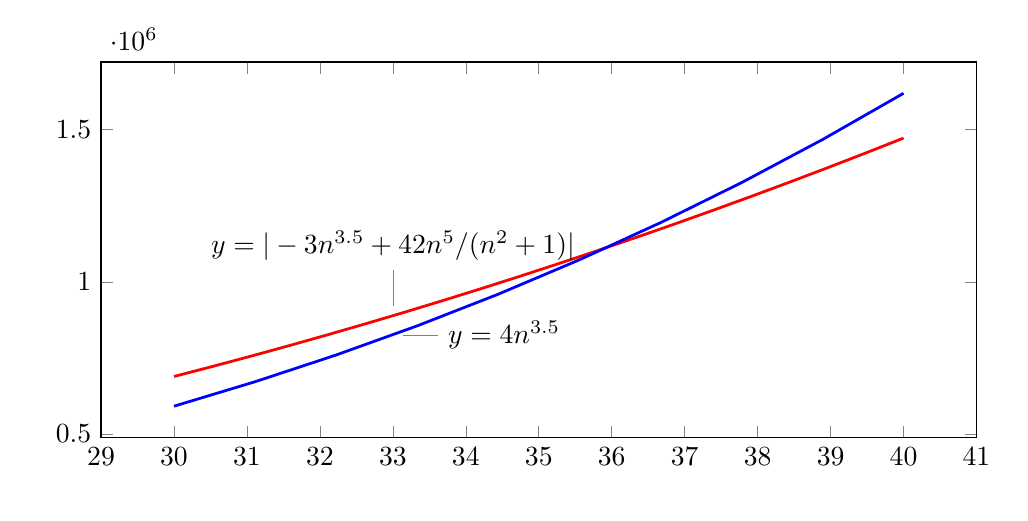
\begin{tikzpicture}[line width=1]
\begin{axis}[width=5in, height=2.5in,
             scatter/classes={a={mark=*,draw=black}},
             xlabel={\mbox{}},
             xlabel style={name=xlabel}, 
             ylabel={\mbox{}}, 
             legend style={
                at={(xlabel.south)},
                yshift=-1ex,
                anchor=north,
                legend cell align=left,
                },
        ]
]
\addplot[draw=red, line width=1] coordinates {(30.0,689086.1269)
(30.5263,721956.7685)
(31.0526,755731.9066)
(31.5789,790416.4277)
(32.1053,826014.9474)
(32.6316,862531.812)
(33.1579,899971.1017)
(33.6842,938336.6319)
(34.2105,977631.9557)
(34.7368,1017860.366)
(35.2632,1059024.8973)
(35.7895,1101128.3279)
(36.3158,1144173.1816)
(36.8421,1188161.7296)
(37.3684,1233095.9925)
(37.8947,1278977.7422)
(38.4211,1325808.5031)
(38.9474,1373589.5543)
(39.4737,1422321.9315)
(40.0,1472006.4278)};\node[pin=above:{$y=|-3n^{3.5} + 42n^5/(n^2 + 1)|$}] at (axis cs:33,888642.2280737216) {};\addplot[draw=blue, line width=1] coordinates {(30.0,591540.3621)
(31.1111,671837.6187)
(32.2222,759633.6609)
(33.3333,855333.7321)
(34.4444,959350.1255)
(35.5556,1072102.0647)
(36.6667,1194015.5915)
(37.7778,1325523.4581)
(38.8889,1467065.0248)
(40.0,1619086.162)};\node[pin=right:{$y=4n^{3.5}$}] at (axis cs:33,825769.3913145486) {};
\end{axis}\end{tikzpicture}\end{center}

If we choose $C = 4$ and $N = 37$,
we see that for $n \geq N$,
\[
\left|
-3n^{3.5} + 42 \frac{n^5}{n^2 + 1}
\right| 
\leq C
\left|
n^4
\right|
\]
i.e.,
\[
|f(n)| \leq C|g(n)|
\]
Hence
\[
f(n) = O(n^4)
\]
\qed
